\section{Conclusions}\label{separation conclusions}

\begin{wrapfigure}{R}{0.4\linewidth}
    \centering
    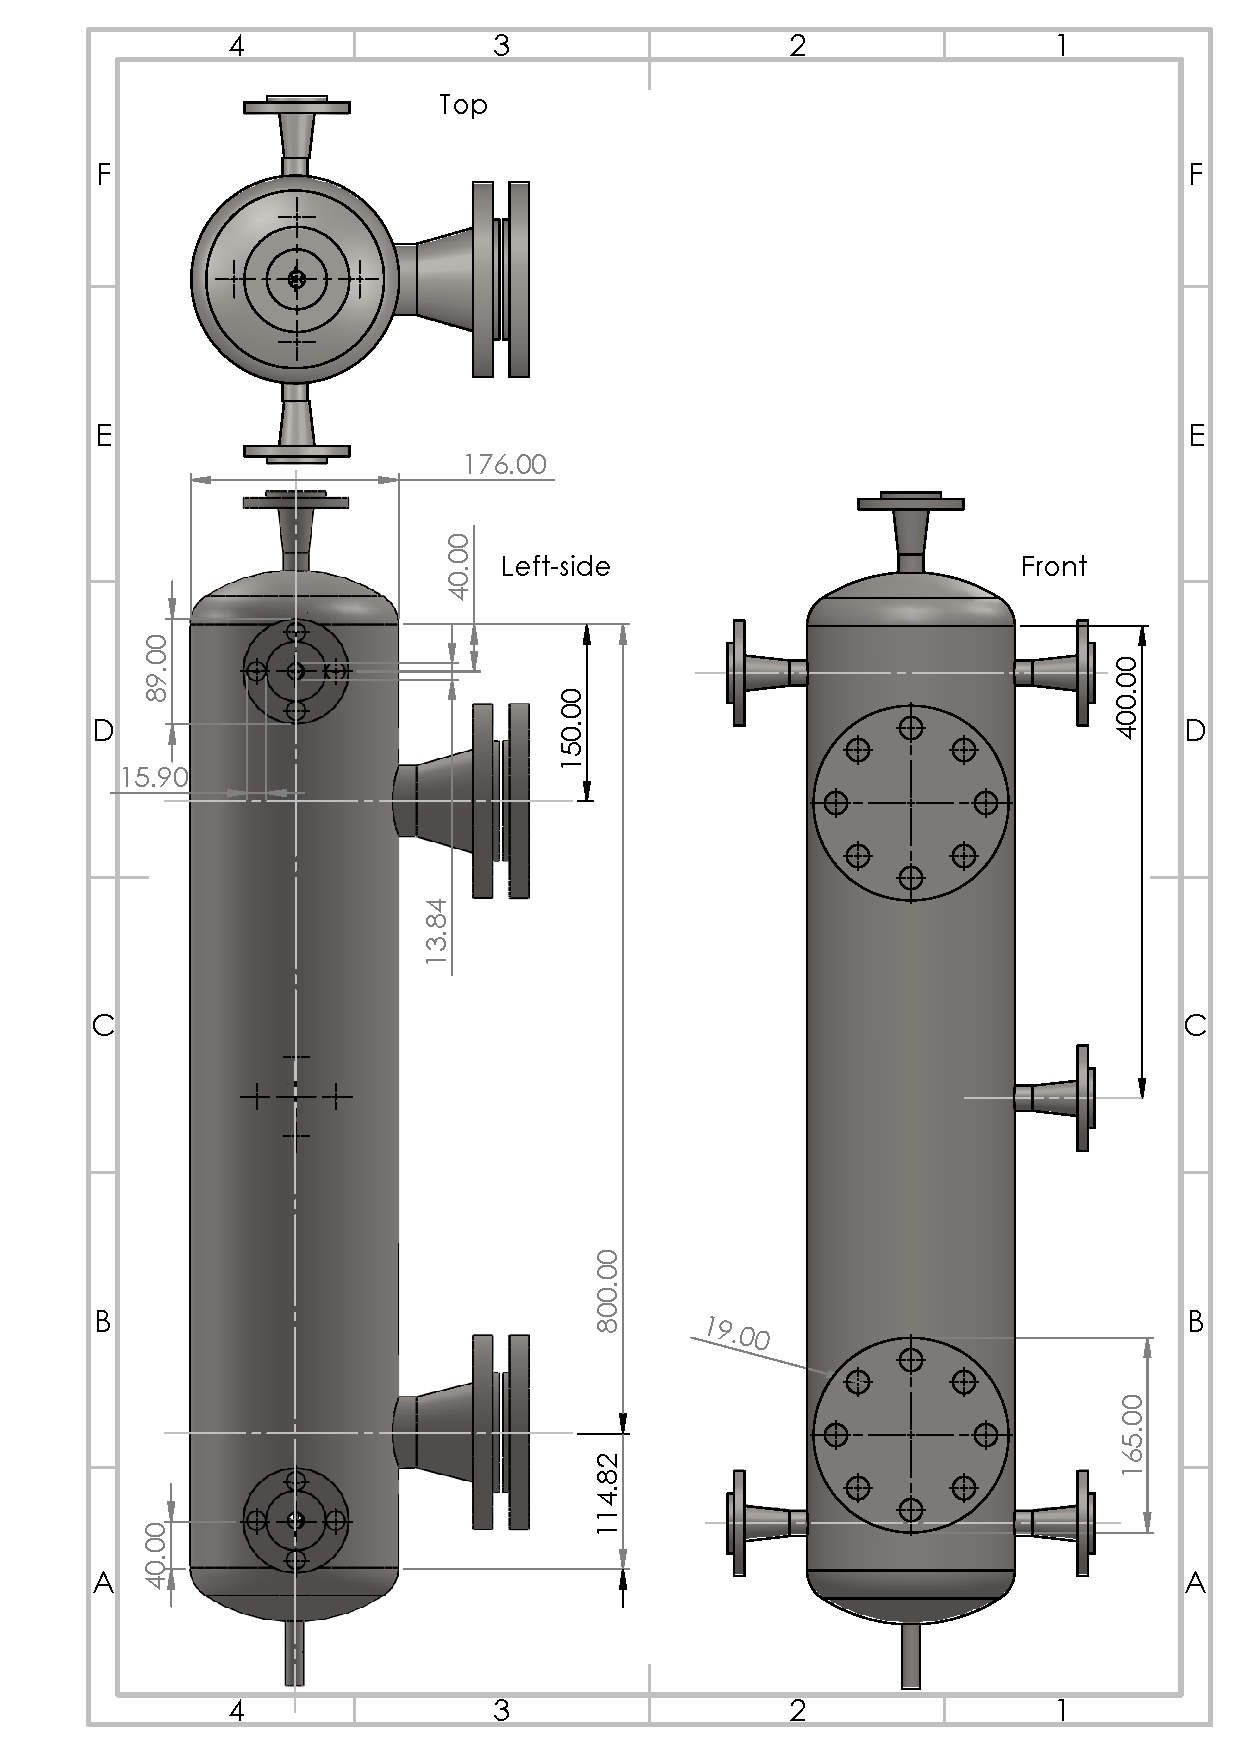
\includegraphics[scale=0.3]{chapters/3-separation/figures/Hydraulic_Wash_Column_GA.PDF}
    \caption{GA drawing for the hydraulic wash column}
    \label{fig:wash column GA}
\end{wrapfigure} 

A separation system has been designed for separating PNT from a mixture of PNT, MNT, and trace of ONT. Crystallisation has been selected as the technique to achieve this separation due to the good difference between the melting points of PNT from MNT and ONT. Distillation, absorption, and adsorption have been deemed inappropriate and hence not selected. The system consists of a MSMPR suspension melt crystalliser, where PNT crystallises as solid, and a hydraulic wash column, where the PNT crystals are separated from the mother liquor and recovered as liquid. 

For the operation of the crystalliser, constant inspection is recommended. With periodic frequency, hot fluid should be run through the cooling coil to melt the fouling caused by PNT solid deposition on the vessel; mechanical cleaning at lower frequency is also recommended. The cooling coil should be chemically cleaned according to a periodic schedule. 


Pilot-scale studies are recommended for a more detailed understanding of the thermophysical processes relevant to the design. The rates of nucleation and growth for crystallisation of PNT from a mixture of PNT and MNT are recommended to be studied. The rate of formation of PNT fouling in the crystalliser should be investigated, where the frequency of periodic inspection and cleaning can be obtained. Assumptions involved in the design of the hydraulic wash column should also be validated. 

\begin{figure}[H]
    \centering
    \includesvg[scale=0.25,inkscapelatex=false]{figures/Wash_column_schematic.svg}
    \caption{Schematics for the hydraulic wash column: (a) perspective (b) left-side section (c) front section (d) section for detailed view of knives (e) section for detailed view of filter tubes crossing.}
    \label{fig:wash column schematic}
\end{figure}

%Crystallisation was used in this separation due the large difference in melting temperatures of the nitro toluene isomers (mainly para and meta) and the requirement for a high purity, high recovery separation step. The crystallisation gave a 90.6\% recovery of PNT solids from the liquid feed mixture. 



%On the issue of fouling, removal mechanisms such as mechanical devices (hammers, scrapers) or chemical removal like the introduction of a solution to dissolve the encrusted layer. Preferably, the removal would be on line to not incur shutdown costs and reduce production, but if necessary, off line techniques could be used.

%Moving forward, pilot studies can be carried out to determine accurate coefficients for crystallisation in both primary and secondary nucleation rather than using the approximate values for similar systems. 